% !TeX root = ./paper.tex
\documentclass[a4paper,12pt]{article}

% Packages
\usepackage[utf8]{inputenc}     
\usepackage{amsmath, amssymb} 
\usepackage{graphicx}          
\usepackage{geometry}           
\usepackage{natbib}   
\bibliographystyle{besjournals}

\usepackage{hyperref}          
\usepackage{subcaption}     
\usepackage{multirow}
\usepackage{float}

% Page layout
\geometry{margin=1in}          

% Title section
\title{TIM: Tree Imaging Machine for low-cost digital images of tree cores and cookies} 
\author{Adam Fong,$^{1}$ Chloe Curry,$^{1}$ Yue Zhang$^{1, 2}$ and E.M. Wolkovich$^{1}$} %emw14Apr2025: You should ask Chloe and Sandy who they want their names displayed (middle initial etc.)
\date{\today}

\begin{document}

\maketitle

\noindent $^{1}$Forest and Conservation Sciences, University of British Columbia, Vancouver, BC, Canada\\
$^{2}$Department of Computer Science and Engineering, University of California San Diego, La Jolla, CA, USA\\ 

%emw24Feb: I added some text to abstract and intro that I am not 100% sure you would need for some journals, but I think you will need for MEE. 
%emw9Mar:

\begin{abstract}  
Studies of tree rings from climatology to ecology have benefitted recently from new methods to image wood rapidly and efficiently, helping to scale up the number and quality of image samples. Current approaches are, however, limited in scanning dimensionality and can be cost-prohibitive. % Getting rid of open-source as CaptuRING is cheap but GigaPixel is expensive and not open source
To address these limitations, we designed the Tree Imaging Machine (TIM)---a do-it-yourself scanning tool to digitize tree cookies and cores. TIM takes partially overlapping microscopic images of samples and stitches the individual images together to form 
a mosaic, which can be zoomed in to visualize features on the scale of 0.01 mm. With scans of up to 21 140 DPI, TIM produces one of the highest resolution images among similar tools for less than \$3 000 USD.
We designed TIM to have a large working plane to allow digitizing cores over 50 cm and complete cookies. Operators can prepare sample batches of multiple cores and cookies, letting the machine work until the queue is finished.

All of the 3D printed parts are available for download on the \href{https://doi.org/10.60705/3DPX/21561.3}{NIH 3D printing repository} and the software is  % is this best practice for including links? 
open source, with instructions to recreate this tool available on \href{https://github.com/temporalecologylab/TreeRings}{GitHub}. TIM provides an important advance in scanning resolution, tree cookie sampling, maximum core sample size, batch digitization, and cost in a single package. This promotes the digitization of larger samples and can collect data at finer resolutions in an open-source design which can be built on and improved as new technologies become available. % Archive GitHub with Zenodo? I'm nervous as the code base is updated relatively frequently... will this be a problem? Or do I only ever make one 'release' https://docs.github.com/en/repositories/archiving-a-github-repository/referencing-and-citing-content 
\end{abstract}

\section{Introduction} %emw9Mar:  edits throughout to tighten things up... please check I did not add typos or nonsensical stuff. 
Incremental growth rings from trees have provided valuable insights into the abiotic and biotic environment across multiple fields---from climatology to forestry and ecology. Dated tree rings from dendrochronology have been critical to
reconstructing past climates of regional and local environments, providing the most accurate, precise, and reliable dating among alternatives \citep{mann_northern_1999}, and thus informing  our understanding of climate change today \citep{fritts_dendroclimatology_1971,williams_using_2010,guibal_dendrochronology_2021,sheppard_dendroclimatology_2010,williams_large_2020}. Tree rings are also increasingly used in ecology to understand how plant competition affects tree growth in addition to climate \citep{buechling_climate_2017} and have implications in forestry to managing stand dynamics \citep{canham_neighborhood_2004}. These fields have leveraged two basic types of tree sampling techniques to capture the variation of tree rings: cores, which are cylindrical samples collected using an incremental borer, and `cookies,' which are entire cross sections \citep[and thus allow measuring as many radii from the sample as desired,][]{speer_fundamentals_2010}. As understanding tree growth and managing forest becomes more critical to mitigating climate change, scaling up the collection and processing of tree ring samples has become increasingly important.

The first computer-based method to measure tree ring widths used a microcomputer, a stage micrometer, and a push button. With this technique, still used widely today, a trained technician shifts a core underneath a microscope objective and pushes a button connected to a microcomputer to record a ring's location \citep{robinson_microcomputer_1980}.
This method has high precision but depends heavily on specific technicians and maintains no image record, preventing later measurement reproducibility and uncertainty quantification \citep{levanic_atrics_2007}.

Image analysis of tree rings was later implemented to reduce both errors in sampling and sampling bias across individual technicians, with major methods developed in the 1980s and 1990s to digitize tree ring samples using optical scanning \citep{mcmillin_application_1982,guay_new_1992}. Optical scanners are still readily available for purchase, using a top of the line scanner (e.g., Epson Perfection V850 Pro) produces a maximum resolutions of 6 400 dpi and scan area of up to 21.6 cm x 29.7 cm.
More recent techniques have aimed to achieve higher resolutions and/or larger samples through a different digitization approach---using an image-capturing system. These systems rely on a microscope camera to take images, motors to move the sample or camera, a computer to manage the capturing, and a second, more powerful, computer to stitch images into a larger composite image.
Decreasing the field of view of each captured image increases the resolution of the final stitched image without restricting the size of the sample \citep{muhlich_stitching_2022}.
Stitching multiple images into one mosaic is a common technique used in other fields such as mineralogy and cellular biology \citep{ro_image_2021,mohammadi_fast_2024}, which was
first implemented for tree rings through the Advanced Tree-Ring Image Capturing System (ATRICS) \citep{levanic_atrics_2007}. % Adding ATRICS after introducing the image and stitch method

Since ATRICS was introduced in 2007, image capture and stitching of tree rings have become more common. Today CaptuRING offers a more modern do-it-yourself alternative to ATRICS, creating scans up to 5 339 dpi using a DSLR camera and motorized stage \citep{garcia-hidalgo_capturing_2022}. 
Another alternative, Gigapixel, achieves an impressive 19 812 dpi with the same DSLR image capture and composite stitch method \citep{griffin_gigapixel_2021}. 
While CaptuRING and Gigapixel both use DSLR cameras and motorized movement, they differ on two fronts. 
First, Gigapixel's camera is traversed across a stationary sample while CaptuRING moves a core sample underneath a stationary camera.
With a mobile camera, multiple samples can be recorded sequentially without needing to remove a sample from a stage upon image completion---significantly reducing the active setup time for an operator. 
Second, Gigapixel automatically stitches individual images together once imaging is complete. This removes the need to transfer images to a more powerful computer for stitching as is necessary with CaptuRING.
Additionally, both of these systems are designed to capture images along a singular axis as the entire width of a core fits within a single image's field of view.
This assumption fundamentally restricts the digitization only to cores, as cookies have a two dimensional scanning surface. %emw9Mar: later 2/3 of paragraph very nice. 

To address some of the current limitations, while building upon the open-source and open-hardware philosophies of CaptuRING with the functionality of Gigapixel, we designed the Tree Imaging Machine (TIM).
We added support to digitize both cookies and cores, increased the maximum sample length, perform image stitching directly without the need for manual file transfer, and capture batches of samples sequentially---all while minimizing cost.
Our design requires the use of 3D printed components and common hand tools such as hex keys and wrenches. No specialized equipment or power tools are required beyond this. 
Excluding 3D printed parts, the total cost of the machine is approximately \$2 200 USD \citep[compared to the \$70 000 USD of the Gigapixel,][]{griffin_gigapixel_2021}.
We chose to use a Raspberry Pi HQ camera with a microscope lens to save on purchasing a professional camera with a macro lens. Professional camera setups are comparable in price to the entire cost of TIM.
These savings combined with not needing to purchase a professional stitching software license (such as PTGui (New House Internet Services BV, Rotterdam, NL), the suggested software to use with CaptuRING) makes TIM a more economical option than most products current available. Additionally the design is open-source and open-hardware allowing for contributors to add new sensors or alter the control methods. 

\section{Methods}

\subsection{TIM System Design} % this is so dry fix later. The engineer in me loves a dry title

\begin{figure}
  \centering
  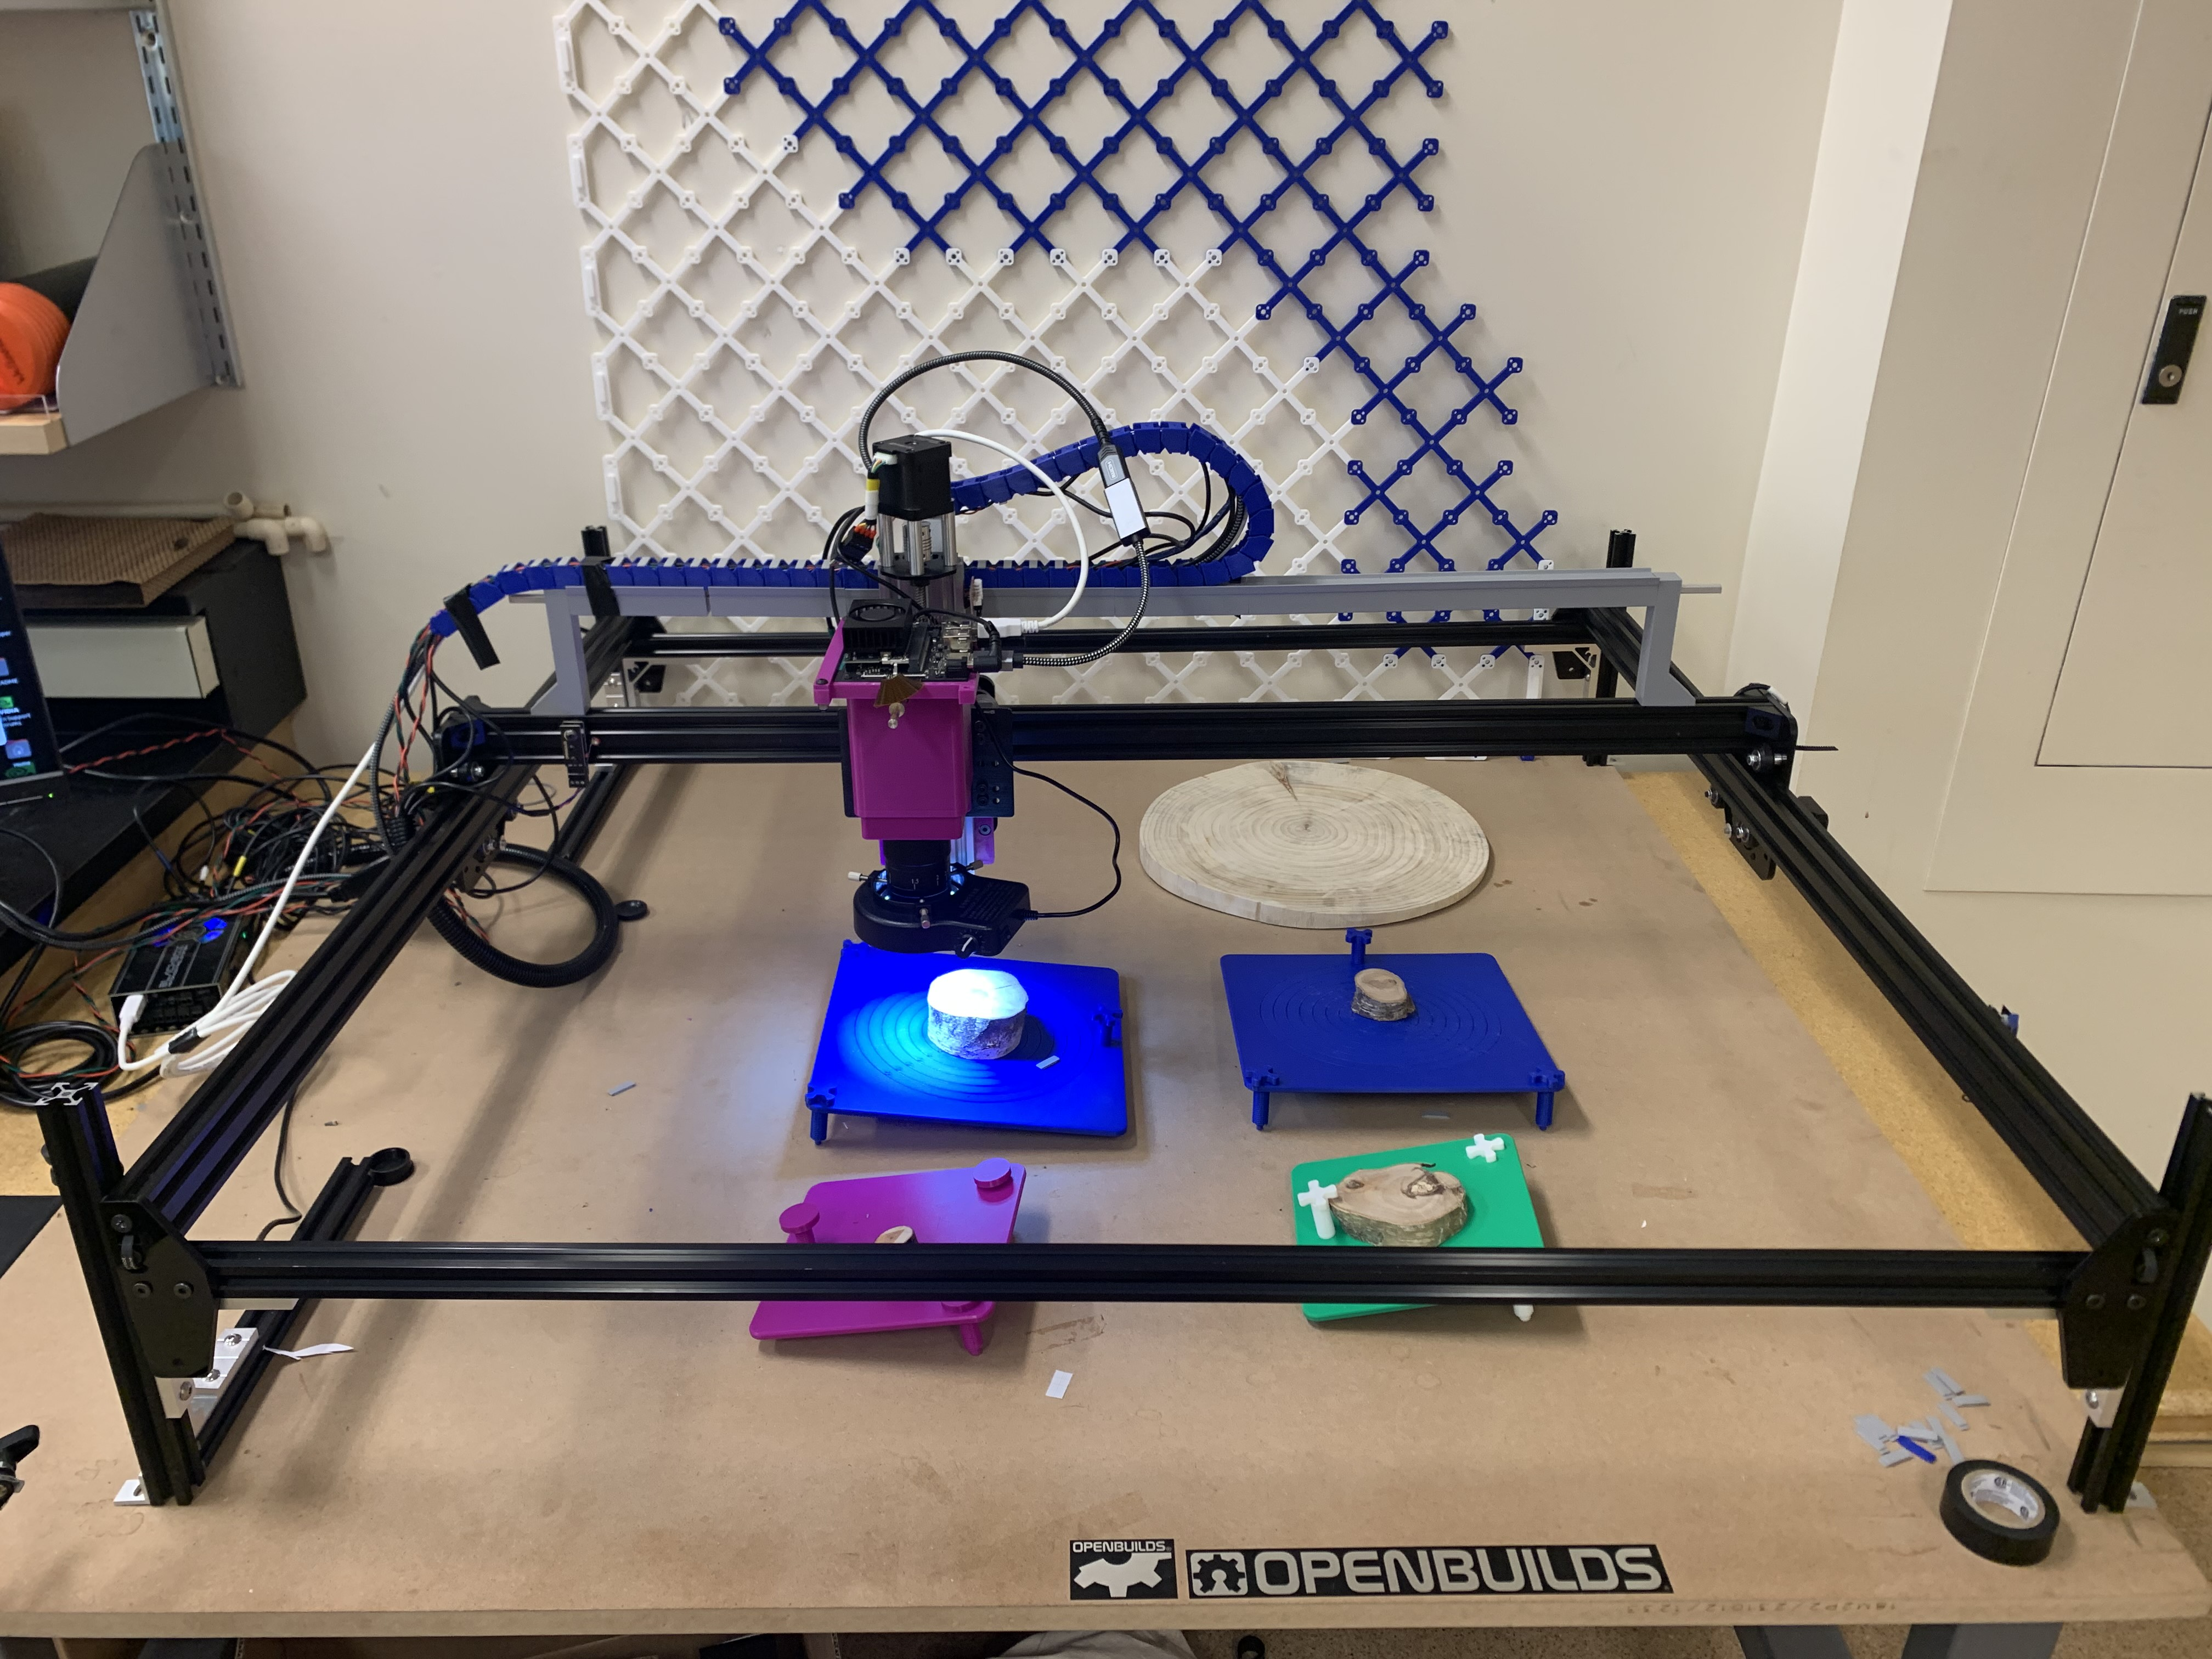
\includegraphics[height=0.5\linewidth]{../content/tina.jpg}
  \caption{Complete assembly of TIM, shown with a few cookies ready to be scanned (in the work plane).}
  \label{fig:tim_assembled}
\end{figure}

% Good topic sentence! Can you walk reader more carefully through each item? You may need to re-order them .. But basically, pick the most useful order and then write: For the camera .... For the gantry machine ... You might also use this space to say, in contrast to previous approaches that have used XX giant camera, we used ... and otherwise point out the novelty when it comes up. 
TIM can be thought of as a combination of multiple subsystems: a gantry machine, camera, and computer (Figure \ref{fig:tim_assembled}). 
For the gantry machine, cartesian movement in the $X$, $Y$ and $Z$ directions is a result of two machine kits and a motor controller from OpenBuilds---the ACRO 1010, the NEMA 17 lead screw linear actuator, and the X32 Motor Controller running GRBL firmware. %vvdm24Apr: I think the Figure 1 could be improve, by indicating the different components (camera, motors...)? I also wonder wheter a schematic diagram would be better than a photo, or maybe at least edit the photo (e.g. remove the wall with the fire extinguisher! Unless, of course, there's a high probability the machine catches fire... :-) )
The machine kit includes extruded aluminum rails, carriages to slide along the rails, stepper motors to control the $X$ and $Y$ movement, and all the hardware to assemble the machine. 
To fit on the build plates of the ACRO system, we made an adapter to connect the linear actuator to the X and Y axis, thus creating motion in the Z axis.
The size of the work plane is ultimately up to the size of the ACRO kit that is purchased---allowing for more flexibility.
Building on top of kits allowed for quick assembly with sound instructions and saved development time. 
For the camera, we chose a 12MP Raspberry Pi HQ Camera equipped with a SEEED studio microscope lens with 150X zoom. The camera was connected to the gantry machine using custom, 3D printed, adapters.
For the computer, we implemented all of the software control, image stitching, and graphical user interface (GUI) to run on an NVIDIA Jetson Orin Nano (Jetson edge computer), which also connects to the camera via a MIPI cable. 
Controlling the machine is done by launching a Python program and interacting with mouse button clicks on the GUI. 

By choosing this combination, we were able to reduce the weight and cost of the camera significantly. This minimized the design challenges of stabilizing the movement of a heavier DSLR and allowed us to invest more in a powerful computer that can handle intensive image processing. 
The Jetson is an edge computer which drives a monitor for a GUI, sends commands to the motor controller to move the machine, runs image processing calculations for control, and performs calculations to stitch individual images into one mosaic. 

\subsection{Preparing Cookies and Cores}
TIM can scan both tree cookies and tree cores. Sample preparation for both are equally important but require different approaches.
The general guidelines used for preparing cookies and cores applies---requiring samples to be sanded with incrementally increasing sand paper grit to produce an even surface for scanning \citep{speer_fundamentals_2010}. We sanded cookies using an orbital sander with mesh sandpaper from 60 to 800 grit, then used a microscope to visually inspect the quality of the sanding. We considered the sample to be sufficiently prepared when vessels were easily identifiable.

TIM requires additional sanding considerations for each sample type. 
For cookies, it is important to have the top and bottom surfaces nearly parallel. 
\begin{figure}
  \centering
  \begin{subfigure}{.5\textwidth}
    \centering
    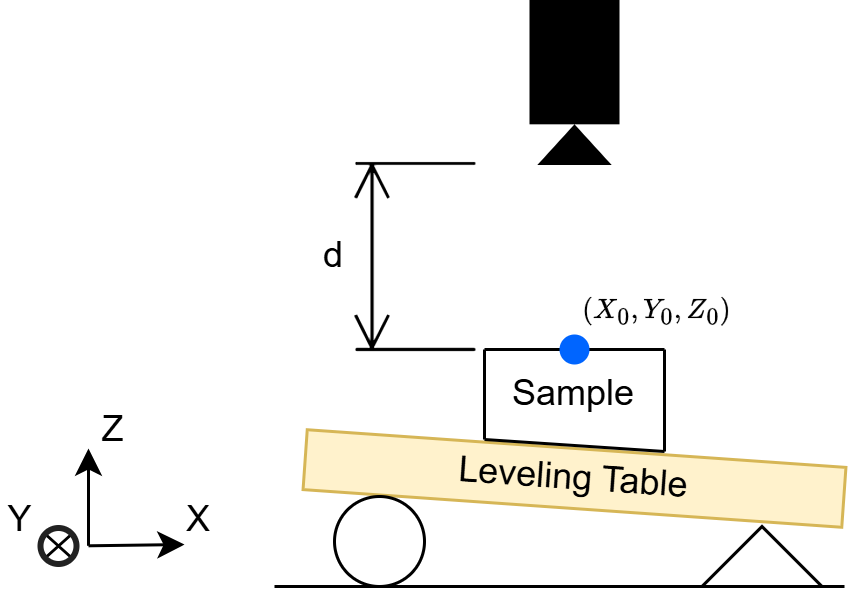
\includegraphics[height=0.5\linewidth]{../diagrams/sample_setup_ideal.png}
    \caption{Ideal sample leveling}
    \label{fig:ideal_levelling}
  \end{subfigure}%
  \begin{subfigure}{.5\textwidth}
    \centering
    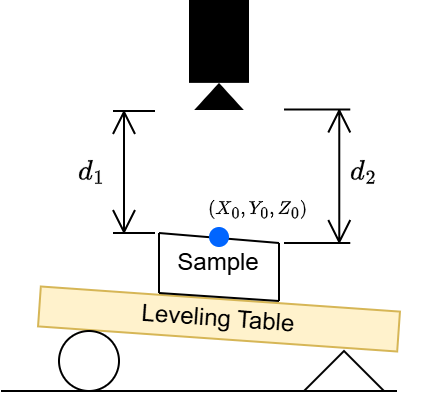
\includegraphics[height=0.5\linewidth]{../diagrams/sample_setup_realistic.png}
    \caption{Realistic sample leveling}
    \label{fig:realistic_levelling}
  \end{subfigure}
  \caption{Side view of the camera (top, in black) and sample on top of a leveling table. The ideal sample leveling shows a uniform distance, $d$, at all $XY$ coordinates on the sample. This is impossible to achieve in reality, the true sample leveling has a non-uniform distance at unique $XY$.}
  \label{fig:sample_levelling}
\end{figure}
Small differences in plane angle can be corrected using the 3D printed leveling table we designed (Figure \ref{fig:ideal_levelling}). 
For cores, care should be taken to maximize the scanning surface. This means removing material to be coincident to the center of the cross section of the core. 
Similarly to cookies, the scanning surface should be as close to parallel to the XY-plane as possible, but generally does not need to be leveled using the leveling tables.
Cores also need to be aligned to be parallel to the $Y$ axis to be digitized, using a squaring tool (or similar) to help with alignment. Any warping in core mounts needs to be counteracted with the use of trigger clamps. 

\subsection{Sample Digitization} % Methods

The subsystems of TIM can be best understood by following the process from sample setup through obtaining a stitched image. 
To achieve this with a fixed focus camera, the samples must be nearly orthogonal to the camera lens. 
Once the sample is level, the operator follows a procedure to inform TIM of where the sample is, and the its size using buttons on the GUI to navigate and focus the camera on the center of the sample. 
The sample height and width in the $X$ and $Y$ dimensions are then entered in the GUI to be saved. Finally, the user must click the `Add Sample' button which provides more fields to add sample identifiers and save the center coordinate.
This procedure can be repeated to create a queue of samples to digitize as a batch. One additional parameter that needs to be defined is the height and width of the field of view of one image from the camera. 
We adjusted the focal length of the camera using the zoom ring to have a constant field of view of approximately 3 mm x 5 mm when in-focus.  
The sample height and width, sample identifiers, sample type, sample center coordinate, and the height and width of an image provides sufficient information to digitize a sample.

\subsubsection{Exhaustive Sample Traverse}  

\begin{figure}
  \centering
  \begin{subfigure}{.3\textwidth}
      \centering
      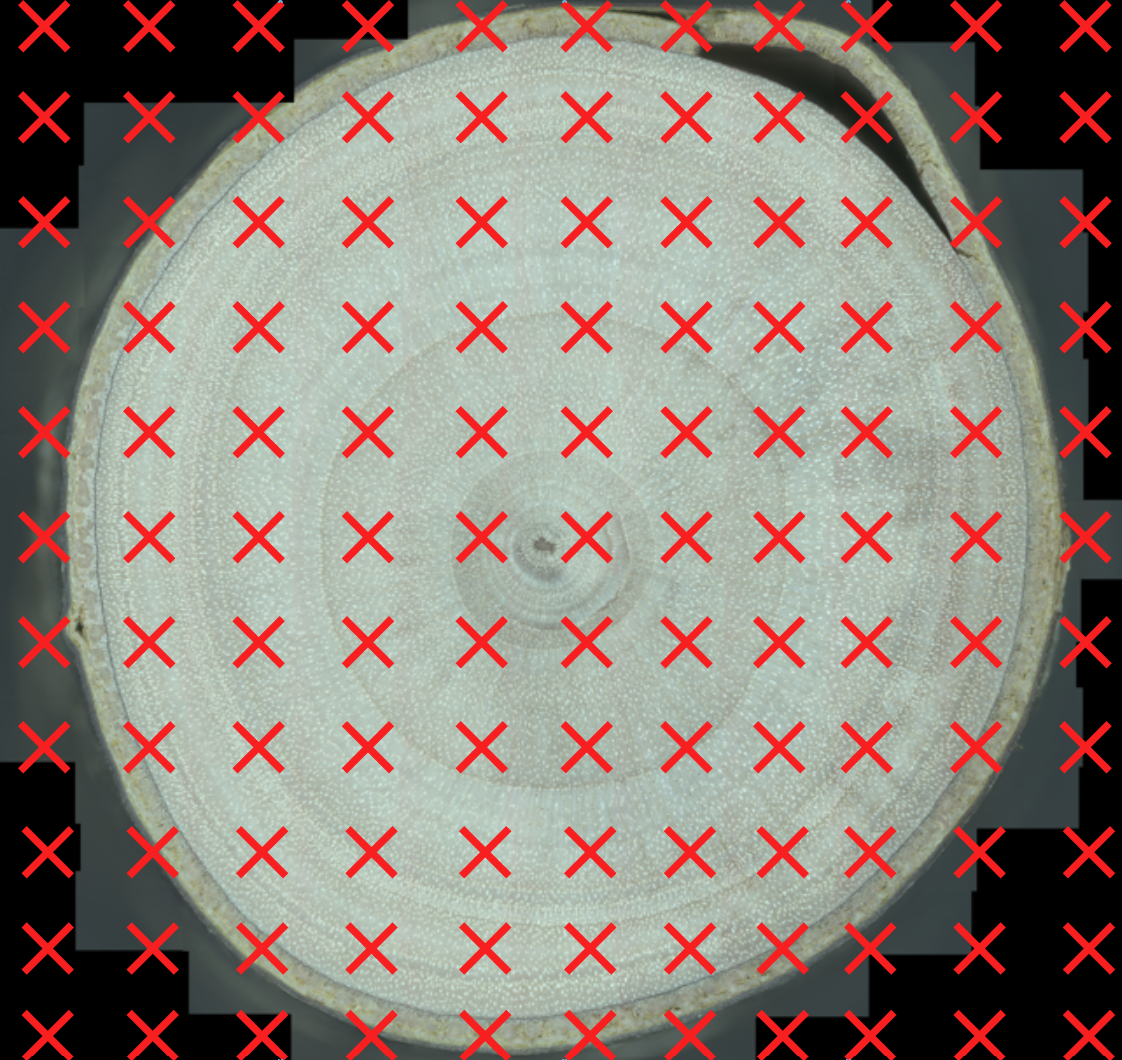
\includegraphics[width=.95\linewidth]{../content/cookie_figure_grid.png}  
      \caption{}
      \label{SUBFIGURE LABEL 1}
  \end{subfigure}
  \begin{subfigure}{.3\textwidth}
      \centering
      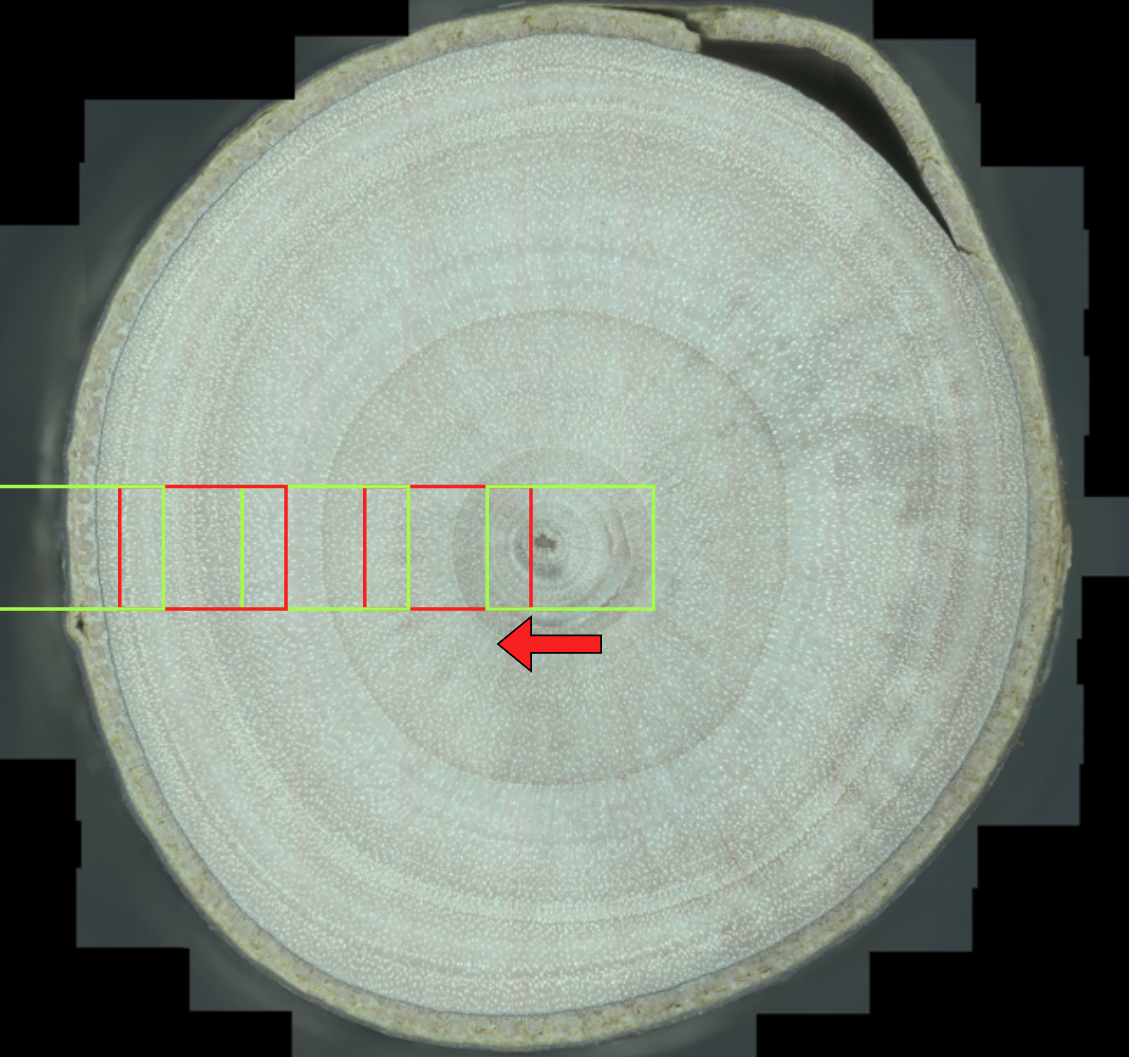
\includegraphics[width=.95\linewidth]{../content/cookie_figure_traverse_start.png}  
      \caption{}
      \label{SUBFIGURE LABEL 2}
  \end{subfigure}
  \begin{subfigure}{.3\textwidth}
      \centering
      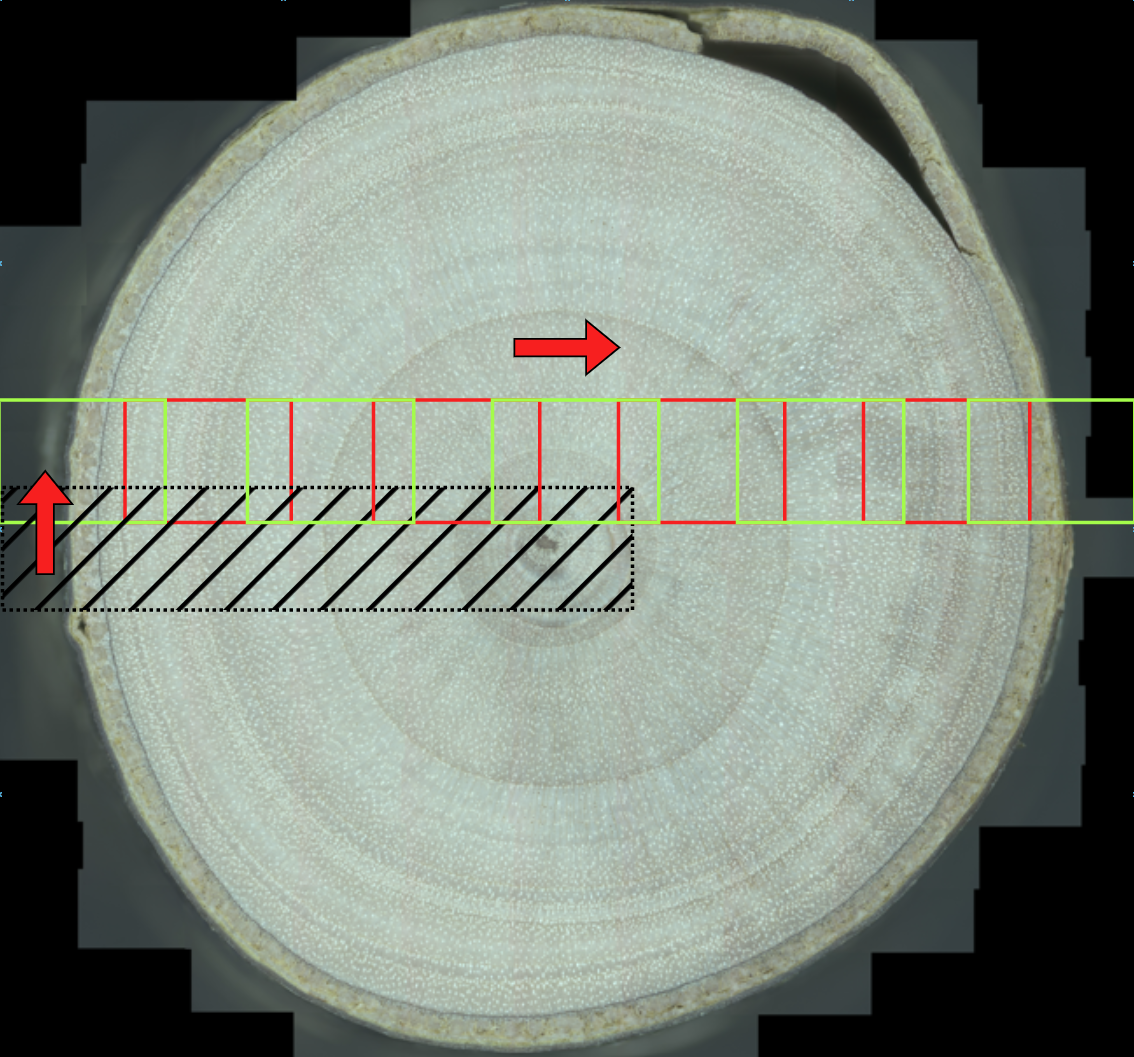
\includegraphics[width=.95\linewidth]{../content/cookie_figure_second_row.png}  
      \caption{}
      \label{SUBFIGURE LABEL 3}
  \end{subfigure} 
  \caption{An example imaging process of a cookie sample. Here, the height and width of the capture region enclose the entire surface area of the cookie.  TIM begins by generating a grid of target coordinates to systematically capture a grid of continuous and partially overlapping images (a). TIM takes its first image at the center coordinate of the sample, then the rectangular field of view from the camera moves to adjacent target coordinates until it reaches the left boundary---capturing an image for each target coordinate (b). After completing the row, TIM moves to a new row and continues capturing adjacent images (c). }
  \label{FIGURE LABEL}
  \end{figure}

The goal of this sample transverse is to obtain in-focus images that have a region of overlap with each of its neighbors---the basis of image stitching (Figure \ref{FIGURE LABEL}). 
The coordinates of each image-to-be-captured are derived from the sample's center coordinate, the height and width of the sample, the height and width of an image frame, and the user provided percentage overlap between images.  
Our design can capture cores by defining the sample width to be zero and the height of the core to be used. So long as the cores are aligned to be parallel to the Y axis, this minimizes imaging time as only one column of images is captured.
Digitizing cookies requires a rectangular grid of images to be taken in both the X and Y axes. 
The user provides enough information to find the X and Y coordinates of each image, but the Z coordinate must be found with an algorithmic focusing procedure. 

\subsubsection{Image Focusing}

With TIM's microscope lens, the depth of field of the image is sensitive enough that sub-millimeter heights can move an image out-of-focus.

This means that the height collected when adding a sample ($Z_0$, we provide a complete glossary of notation used to describe the methods, see Table \ref{tab:math_notation}) does not produce in-focus images throughout the entire surface area of the sample.
To capture an in-focus image at height $Z_{focused,k}$, for each unique image coordinate $(X_k, Y_k)$, we implemented a time-conscious software procedure. 
Our procedure involves two stages and starts at the known center coordinate of the sample.
The first stage takes advantage of the requirement that the sample is in-focus when adding it to be scanned.
Starting at the center coordinate allows the initial $Z_0$ value, captured when adding a sample, to find $Z_{focused,0}$. 
After finding an in-focus image, TIM navigates to the next neighboring image coordinate to find its in-focus image, using the previous neighbor's in-focus height as an initial approximation.

Finding an in-focus image is completed by comparing the image sharpness of a set of images at varying heights (a vector $\boldsymbol{Z_k}$) but the same coordinate $(X_k, Y_k)$. 
The differences in height between each image are equally spaced, and are described by the relative distance to the starting height, $Z_k$, in the vector $\boldsymbol{\delta}$. 
We found that it is important to have a distance of no more than 0.1 mm between each image in the stack of images to maximize the likelihood of an in-focus image at height $Z_{focused,k}$.
A height range of 1 mm provides a sufficient distribution of image sharpness. TIM needs to take 11 images at different heights to navigate this height range with the given step size between each image. The number of images taken is an editable parameter in the configuration file and can be increased, along with the height range, if TIM Is not obtaining in-focus images.

Our focusing procedure begins at 0.5 mm above $Z_k$ and finishes with the last image at 0.5 mm below $Z_k$.
The 11 images then have their normalized variance calculated in a separate thread to measure the image sharpness \citep{sampat_extensive_2014}.
The image with the maximum score is saved and can be considered the most in-focus image, while the rest are deleted. 
Now $Z_{focused,k}$ has been found for $(X_k, Y_k)$ and the camera can now be moved to the next image coordinates $(X_{k+1}, Y_{k+1})$ and repeat the process to find a new in-focus height.

The second stage of our time-efficient focusing procedure uses a feedback loop to update the initial $Z_k$ at each image location $(X_k, Y_k, Z_k)$. 
Without a feedback loop, the sample alignment must have a difference in height no greater than 0.5 mm ($d_1 - d_2 < 0.5\,\text{mm}$ in Figure \ref{fig:realistic_levelling}). 
Rather than increasing this height range, a greater alignment error can be managed by adjusting the starting image height until $Z_{focused,k}$ is at the center index of $\boldsymbol{Z_{samples,k}}$. 
The likelihood of an adjacent image, at the coordinate $(X_{k+1}, Y_{k+1})$, containing an in-focus image is highest in this scenario. 
A negative feedback  
proportional-integral-derivative (PID) control algorithm is used to adjust the initial height of each image, with $\alpha_k$, whenever the camera moves in the X or Y dimensions \citep{odwyer_summary_2000}. 
This alleviates the need of having remarkably level sample alignment ($d_1 - d_2 < 0.5\,\text{mm}$ in Figure \ref{fig:realistic_levelling}). 
\[
Z_k = \begin{cases}
  Z_0 & \text{if } k = 0,\\
  Z_{k-1} + \alpha_k \\
  \end{cases}
\]
\[\boldsymbol{\delta} = 
\begin{bmatrix}
  0.5 \\
  0.4 \\
  \vdots \\
  -0.4 \\
  -0.5 \\
  \end{bmatrix}\]
\[
Z_{focused,k} \in
\boldsymbol{Z_k} = 
Z_k + \boldsymbol{\delta}
\] 

To reduce motion blur in the images, the range of $\boldsymbol{Z_k}$ is traversed at constant velocity and images are captured without stopping. 
Decoupling the auxiliary camera control from the G-code commands to control the machine has shown to decrease digitization time and decrease vibrational effects from acceleration and deceleration \citep{propst_time_2025}.
This is a variation of the standard approach used in 3D printing and Computer Numerical Control (CNC) machining. 
  
\subsubsection{Accounting for Translation Error Between Core Samples}

Difficulties arise when more than one core are added to the digitization queue.
The ACRO has a theoretical 4.5 micron translational accuracy, but has not been achieved despite significant effort.
These inaccuracies can cause drift in the images with relation to the core and result in the width of the core not being within the field of view of the images.
We thus implemented a centering procedure that realigns the center of the core to the center of the image frame when the machine moves 
to a new sample. 

First, the camera is moved to the initial coordinates of the camera when the sample is first saved by the user $(X_0, Y_0, Z_0$, Table \ref{tab:math_notation}) of the new core. 
From there, the camera is moved across a window, at constant velocity. %emw9Mar:  w is introduced nicely below. Need to try to follow this format when possible. 
The width of the window, $w$, in millimeters is defined in the machine configuration file and is editable %emw9Mar:  we need a noun below ...
(from $X_0 - 1/2*{w}, Y_0, Z_0$ to $X_0 + 1/2*{w}, Y_0, Z_0)$. 
Images are captured at equal distance intervals analogously to the image focusing procedure. 
Once again, the image with the highest normalized variance score is considered the best image and its location is used as the realigned $X_0$.
This procedure drastically improves digitization quality of batches of cores.

\subsubsection{Stitching}

Image stitching is a well explored field, ranging from panoramic images taken on smart phones to highly tuned microscopy slide stitching. 
Stitching one image to another requires both to share a region of overlap. When capturing a sample using TIM, the operator has the ability to choose a percentage amount of overlap between images.
Most samples are digitized with a percentage overlap between 33\% and 50\%.

After testing numerous image stitching software APIs, we found the Python package Stitch2D most capable of stitching our images successfully. % need to reference this
This package wraps OpenCV functions for finding distinctive image features using the SIFT feature detector and matches these features within the overlapping region of adjacent images \citep{lowe_distinctive_2004}. 
The default implementation of the package produces high quality stitches but is memory inefficient. %is this wording correct?, I'm trying to kindly say it was memory inefficient
We implemented a few key memory-conscious changes such as loading only one image into RAM at a time and writing the final image to a memory-mapped NumPy file before converting to a TIFF file. These changes allowed for the package to run on a Jetson edge computer without a problem.

Some tree ring analyses may not need the maximum scanning resolution produced by TIM. At maximum resolution, TIM's scans quickly produce large file sizes and can be costly to store at scale. 
To address this, a parameter in the machine configuration file allows the operator to choose a downsizing ratio to apply to images before they are stitched, decreasing the file size of the scans.
With the same images, multiple final stitched resolutions can be made. 

\section{Results \& Discussion} 
%emw9Mar: I wondered about this being Results & Discussion ... would MEE be okay with that? It would work better for the paper I think. What do the guidelines say on formatting for articles? 
% MEE's guidelines have a distinct Results section from Discussion although maybe they're flexible on this? Conclusion is optional for MEE



TIM is capable of producing extremely high resolution scans. We calculated the maximum dots per inch (DPI) at 21 140 of individual images captured from the system using a microscopy slide scale (with 0.01 mm graduations, Figure \ref{fig:dpi_measurements}), and developed a Python tool to replicate this for varied lens focal lengths. When downscaling the final stitch, 
DPI scales linearly with the downscale percentage defined in the machine parameters. 

Digitizing samples takes significantly longer for cookies than it does for cores (Figure \ref{fig:digitization_time}). This is due to the surface area of cookies requiring more images as it has a square relationship to sample radius.
For large cookies, the operator can choose to selectively scan a radius of the cookie instead of the whole surface. A single radius contains a portion of each ring. Scanning complete cookies at maximum DPI is unrealistic as file size limits are quickly encountered with small diameter cookies. 

To fit into the maximum 2.5 GB limits of a TIFF file, the maximum diameter of a cookie scanned at 30\% of maximum resolution is limited to approximately 130 mm. This maximum cookie diameter is significantly smaller than the maximum core sample length. At maximum resolution, the file size limit 
constrains core samples to approximately 1 500 mm in length (though a larger ACRO frame than shown here would be needed to support this sample length). Samples larger than this limit can still be scanned, but TIM saves them as an uncompressed binary NumPy memory-mapped array file is produced. Currently, NumPy files are not supported by standard image viewers like ImageJ and would require custom tools to work with. %emw9Mar: Like custom Python scripts? I think we might be more explicit here if we mean that. 

\begin{figure}
    \centering
    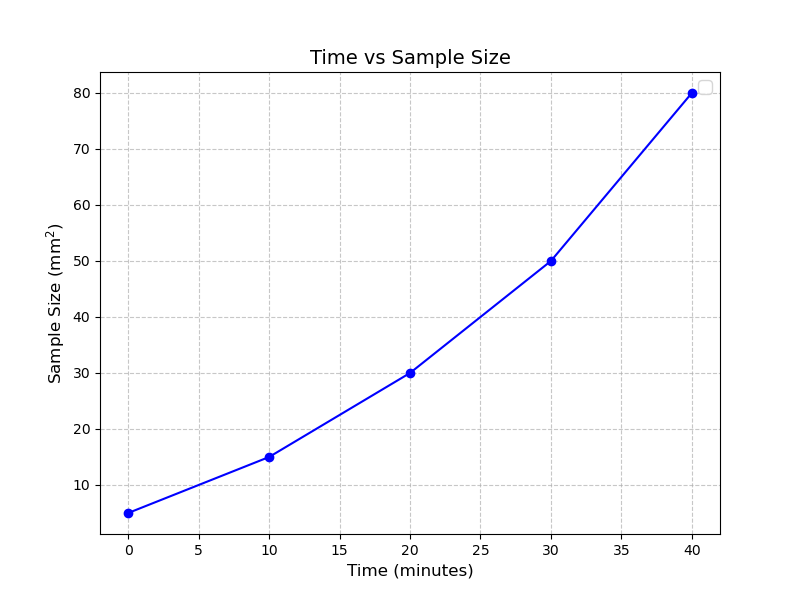
\includegraphics[height=0.5\linewidth]{../../code/plots/time_and_area.png}
    \caption{Time to digitize a sample is dependent on the sample's surface area and the desired final resolution.
    Cores benefit from linear surface area to sample length. The range of sample included are from a 3mm x 220mm core to a 75mm x 56mm cookie. True sampling times are drastically influenced by configurable machine parameters.} 
    \label{fig:digitization_time}
\end{figure}

\subsection{Strengths and Opportunities} %emw9Mar: And this section could become part of the Results & Discussion.... 
% add better opportunities
TIM's design minimizes the barriers to build an affordable, efficient and high-resolution image capture system in smaller labs without compromising scan quality, and while allowing scanning of cookies and cores. We have measured tree ring widths using the digitized samples from TIM using CooRecorder as well as ImageJ \citep{schneider_nih_2012}. 
%emw9Mar: Any citations for developing repos to share tree ring images? Or just more on building better open shared data for tree rings? 
% It appears databases store data after images are processed and measured, potentially too expensive to store image datasets at high resolution?
Publicly available tree-ring datasets can be found on multiple online repositories such as TreeSource's Tree-Rings Database for Canadian sites or the International Tree-Ring Data Bank (ITRDB) for worldwide data \citep{girardin_national_2021} \citep{grissino-mayer_international_1997}.
Both of these databases offer metadata-rich data on measured tree-rings but do not store the source images of samples.
One opportunity for this development could come as more universal and large-scale open-data storage of tree ring images come online. 
Such open repositories would also increase the value of developing new frameworks count vessel or identify rings, which are already starting and have the potential to greatly decrease the time invested in manually identifying tree anatomy \citep{resente_mask_2021} \citep{polacek_automation_2023}. 
With these more fully developed TIM could be extended to be run such frameworks while scanning, possibly taking additional scans only when needed to reach sufficient algorithm accuracy. %emw9Mar -- check my riffing here. 

In its current state, TIM only provides scanned images and requires users to import them into other tools for additional visual analyses, such as measuring tree-ring widths or counting vessels.
A useful addition to TIM would be to automatically detect tree-ring widths or other metrics while capturing images using computer vision models. We expect this may be possible as these methods improve in efficiency. Currently, we found that tree-ring detection by a recent machine learning algorithm  \citeauthor[R-CNN presented by][]{polacek_automation_2023} for a scanned core (23294 x 897 pixels) took 15 minutes on a high-performance cluster (UBC ARC Sockeye) and 3.5 hours on a smaller server (RTX A6000 GPU server). 
Although the Jetson edge computer is not as powerful as these servers, running these models in parallel to the image capturing algorithms would further reduce manual data annotation of tree-rings, and thus could help scale-up data collection.

An additional major frontier for machines such as TIM is integrating additional sensors. While much of the current imaging time of samples comes from taking a vertical stack of images to obtain one in-focus image, advanced microscopy applications have overcome similar challenges through supplemental sensors that measure the distance between the subject and lens.
Adding such sensor support and a control loop to focus images could significantly reduce sampling time on the scale of an order of magnitude. 
Using rotary encoders on each of the motors controlling the X and Y movement would be a welcomed addition---this would greatly increase the 
accuracy of the the location of the camera on the work plane.  

\section{Conclusion} % I think we could remind the reader here of what gaps TIM addresses, but I can help do that next time.  %emw9Mar: This section could move down and become conclusions if we merge the Results & Discussion. 
By taking advantage of a common three degree of freedom cartesian machine design, powerful edge computing, and a microscope camera we were able to design a cost effective and high resolution digitization tool for wood samples. 
Our design significantly increases the maximum sample length and maximum resolution compared to common alternatives in the field. 
In addition, the machine design was intended to be readily replicated by labs with minimal engineering experience and equipment. 
Such an open-source device could facilitate the widespread sampling of tree rings across diverse ecosystems and reduce barriers for researchers with tight budgets. 

%emw14Apr2025: Add acknowledgments here: Deirdre, Hoai Huong Nguyen Phan, Fredi, CRD, Mao etc. 

%vvdm24Apr: and also something like "It will also support tree-ring research in countries where budget constraints may limit access to more expensive equipment..."?

%vvdm24Apr: More general comment: I think it would be helpful to further justify (from an ecological perspective) why high-resolution scans are necessary? Not only to better distinguish the rings, but also for example to differentiate early wood and late wood... or something else (I'm not an expert)? 
\section{Acknowledgments}
The authors thank Deirdre Loughnan, Hoai Huong Nguyen Phan, Frederik Baumgarten for conversations and ideas to help bring this project to fruition. Additionally, we thank Xiaomao Wang and Christophe Rouleau-Desrochers for their help and patience in operating TIM during development. 

\section{Supplemental Information}

{
\renewcommand{\thefigure}{S\arabic{figure}}
\setcounter{figure}{0}  % Start supplemental figures from S1

\begin{figure}[htbp]
  \centering
  \begin{subfigure}{.5\textwidth}
    \centering
    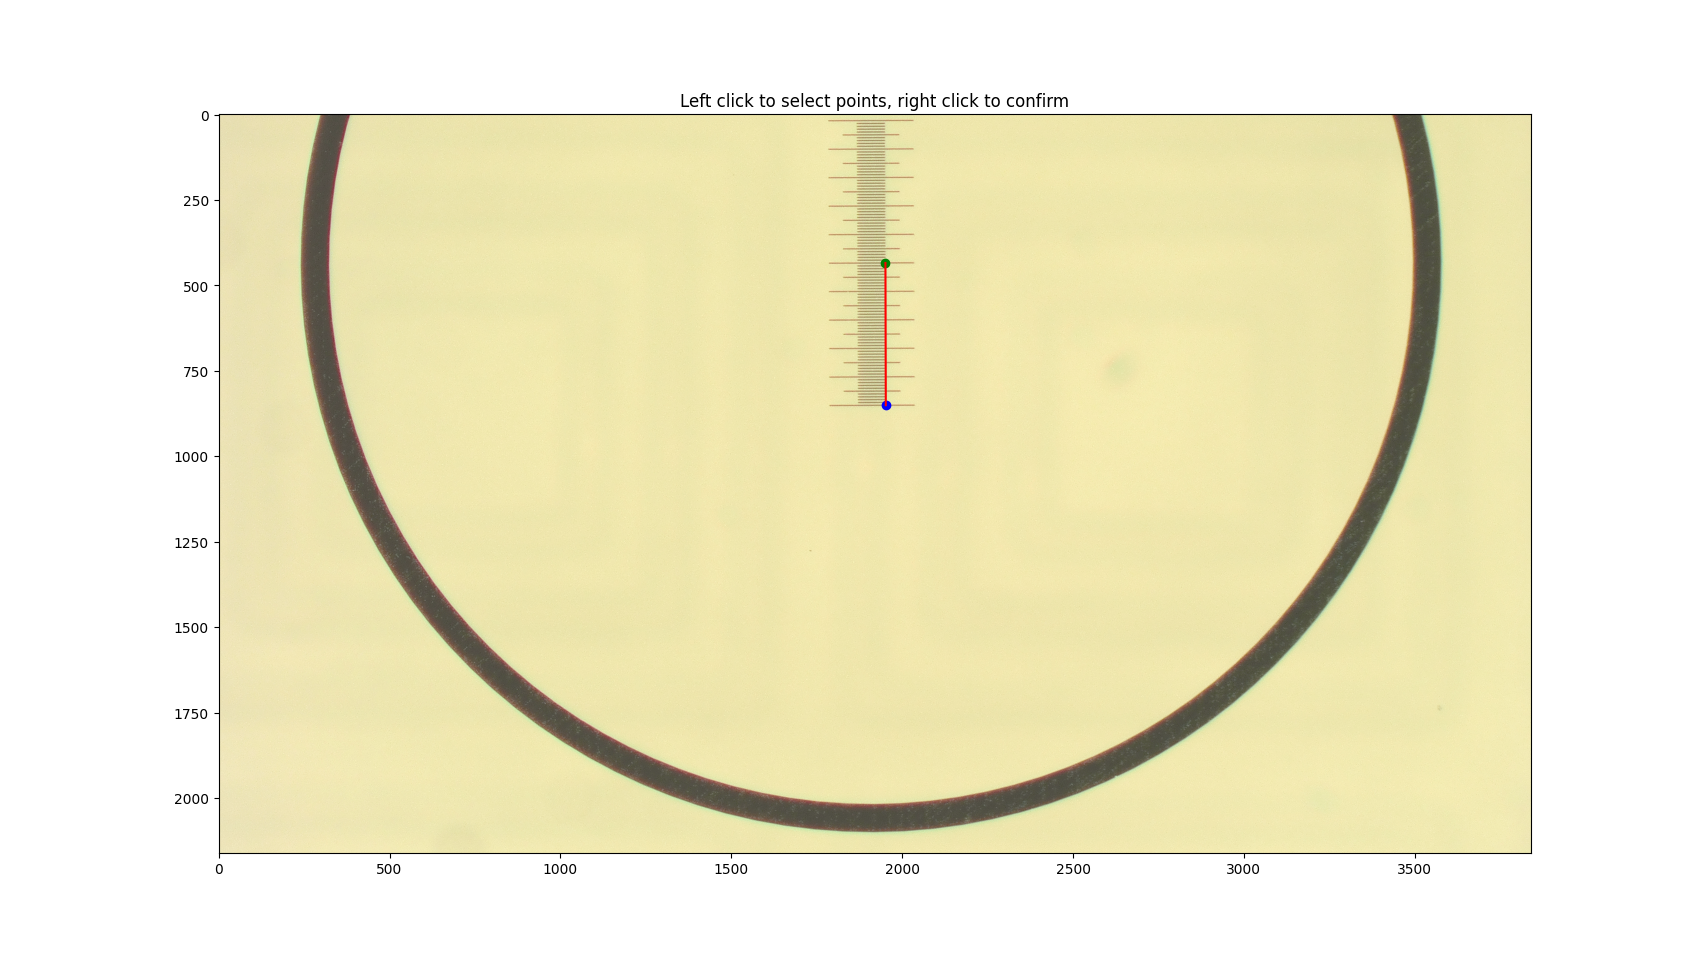
\includegraphics[height=0.5\linewidth]{../diagrams/dpi_measurement_whole.png}
    \caption{Scale Bar for DPI measurements}
    \label{fig:dpi_measurement_whole}
  \end{subfigure}%
  \begin{subfigure}{.5\textwidth}
    \centering
    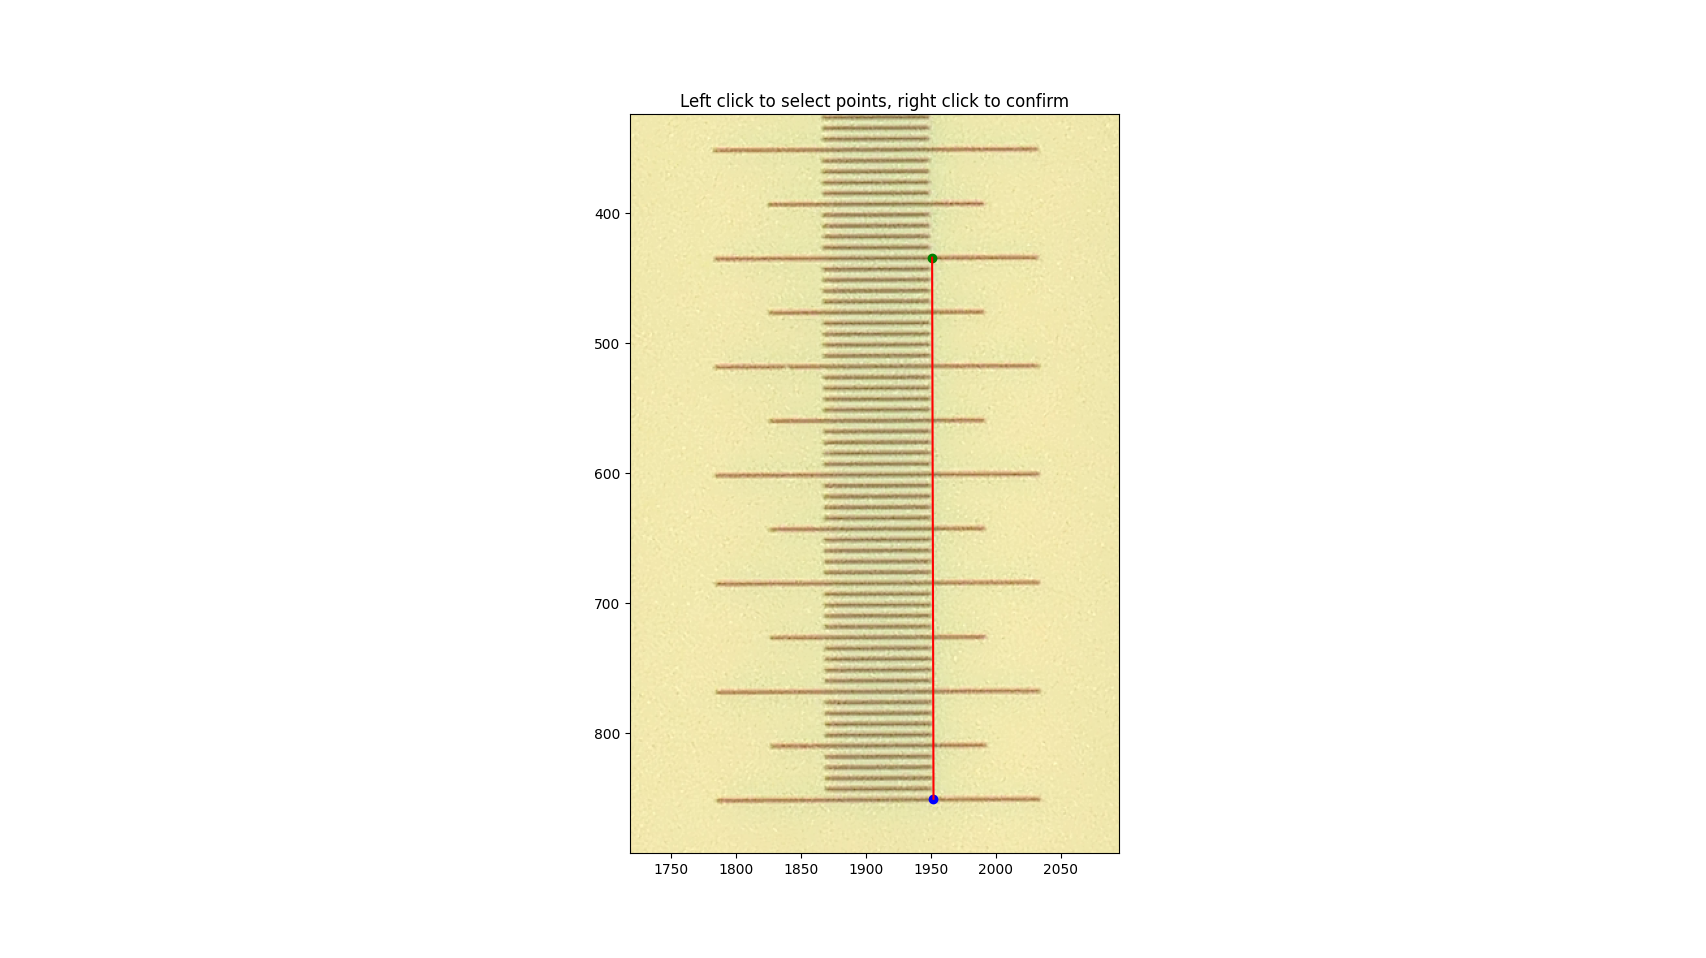
\includegraphics[height=0.5\linewidth]{../diagrams/dpi_measurement_zoomed_2.png}
    \caption{Zoomed in Scale Bar}
    \label{fig:dpi_measurement_zoomed}
  \end{subfigure}
  \caption{Example of a single DPI measurement using a 0.01 mm slide scale. We found the DPI measured at multiple locations in the field of view vertically and horizontally converged on the same value.}
  \label{fig:dpi_measurements}
\end{figure}
}

\renewcommand{\thetable}{S\arabic{table}}
\begin{table}[htbp]
    \centering
    \label{tab:math_notation}
    \begin{tabular}{ |p{3.5cm}||p{11.5cm}|  }
      \hline
      % \multicolumn{2}{|c|}{Math Notation} \\ %emw14Apr2025 -- remove this line -- you just need the caption and then the table should start immediately
      \hline
      Terms & Definition\\ 
      \hline
      $X_0, Y_0, Z_0$   &The initial cartesian coordinates of the camera when the sample is saved by the user. \\
      $Z_k$ & The center height of $\boldsymbol{Z_k}$ which was the best approximation of $Z_{focused,k}$ from the previous image.\\ 
      $(X_k, Y_k, Z_{focused,k})$ & A unique set of $X$, $Y$, and $Z$ coordinates for a unique image of the sample, $k$. \\
      $(X_{k+1}, Y_{k+1})$ & The $X$ and $Y$ coordinates of an image that neighbors image $k$ at $(X_k, Y_k)$. \\
      $\boldsymbol{\delta}$ & Equally spaced heights, relative to $Z_k$, to capture images at and use to find a sharp image. \\
      $\alpha_k$ & The response variable of the PID control algorithm which adjusts the initial height of an image to gradually align $Z_{focused,k}$ to be at the center index of $\boldsymbol{Z_k}$.\\
      $Z_{focused,k}$ & The $Z$ value of the most in-focus image in $\boldsymbol{Z_k}$. \\
      $Z_{focused,0}$ & The $Z$ value of the center coordinate, and first image of the sample. \\
      $\boldsymbol{Z_k}$ & A vector containing the $Z$ coordinates for multiple images at the same $(X_k, Y_k)$. \\
      $w$ & The width of the window to traverse when trying to center a core. \\
      $d_1$ & The relative distance from the camera to one edge of a leveled sample (Figure \ref{fig:sample_levelling}).\\
      $d_2$ & The relative distance from the camera to the opposite edge of a leveled sample (Figure \ref{fig:sample_levelling}). \\
      \hline
    \end{tabular}
    \caption{Mathematical notation used in this paper.} %emw14Apr2025: Explain what the bolding means
    \end{table}
    

\bibliography{references}

\end{document}
